\section{Co-de Bruijn representation, cooked two ways}\label{sec:codebruijn}


%<*named>
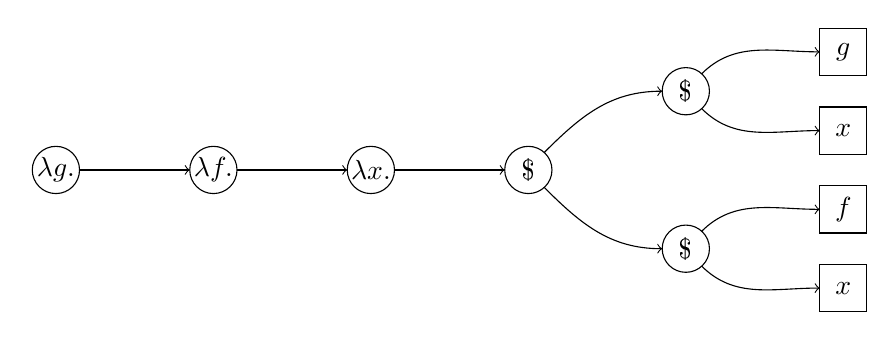
\begin{tikzpicture}
\draw (0,0) circle (.3cm) node[align=center] {$\lambda{}g.$};
\draw (2,0) circle (.3cm) node[align=center] {$\lambda{}f.$};
\draw (4,0) circle (.3cm) node[align=center] {$\lambda{}x.$};

\draw (6,0) circle (.3cm) node[align=center] {\$};

\draw (8,1) circle (.3cm) node[align=center] {\$};
\draw (10,1.5) node[align=center] {$g$} +(-.3cm,-.3cm) rectangle +(.3cm,.3cm);
\draw (10,.5)  node[align=center] {$x$} +(-.3cm,-.3cm) rectangle +(.3cm,.3cm);

\draw (8,-1) circle (.3cm) node[align=center] {\$};
\draw (10,-.5)  node[align=center] {$f$} +(-.3cm,-.3cm) rectangle +(.3cm,.3cm);
\draw (10,-1.5) node[align=center] {$x$} +(-.3cm,-.3cm) rectangle +(.3cm,.3cm);

\draw [->] (0.3,0)     to [out=0,in=180]   (1.7,0);
\draw [->] (2.3,0)     to [out=0,in=180]   (3.7,0);
\draw [->] (4.3,0)     to [out=0,in=180]   (5.7,0);
\draw [->] (6.2,-.22)  to [out=-45,in=180]  (7.7,-1);
\draw [->] (6.2,.22)   to [out=45,in=180]  (7.7,1);
\draw [->] (8.2,1.22)  to [out=45,in=180]  (9.7,1.5);
\draw [->] (8.2,.78)   to [out=-45,in=180] (9.7,.5);
\draw [->] (8.2,-1.22) to [out=-45,in=180] (9.7,-1.5);
\draw [->] (8.2,-.78)  to [out=45,in=180]  (9.7,-.5);
\end{tikzpicture}
%</named>

%<*debruijn>
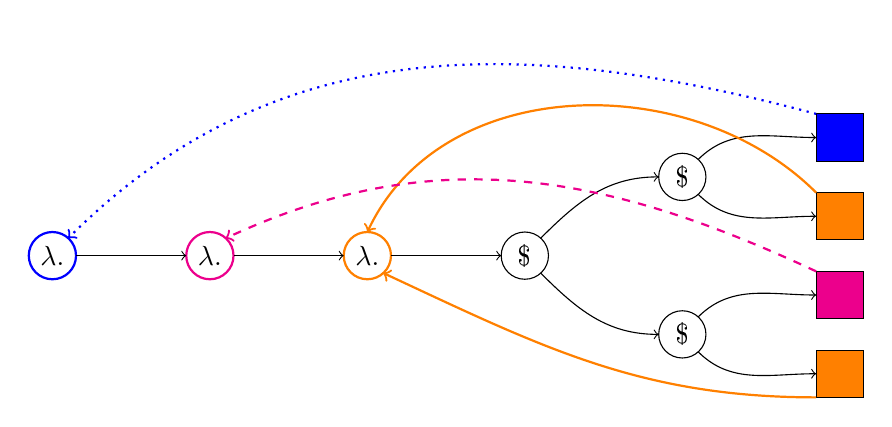
\begin{tikzpicture}
\draw[draw=blue   ,thick] (0,0) circle (.3cm) node[align=center] {$\lambda{}.$};
\draw[draw=magenta,thick] (2,0) circle (.3cm) node[align=center] {$\lambda{}.$};
\draw[draw=orange ,thick] (4,0) circle (.3cm) node[align=center] {$\lambda{}.$};

\draw (6,0) circle (.3cm) node[align=center] {\$};

\draw (8,1) circle (.3cm) node[align=center] {\$};
\draw[fill=blue]   (10,1.5) +(-.3cm,-.3cm) rectangle +(.3cm,.3cm);
\draw[fill=orange] (10,.5)  +(-.3cm,-.3cm) rectangle +(.3cm,.3cm);

\draw (8,-1) circle (.3cm) node[align=center] {\$};
\draw[fill=magenta] (10,-.5)  +(-.3cm,-.3cm) rectangle +(.3cm,.3cm);
\draw[fill=orange]  (10,-1.5) +(-.3cm,-.3cm) rectangle +(.3cm,.3cm);

\draw [->] (0.3,0)     to [out=0,in=180]   (1.7,0);
\draw [->] (2.3,0)     to [out=0,in=180]   (3.7,0);
\draw [->] (4.3,0)     to [out=0,in=180]   (5.7,0);
\draw [->] (6.2,-.22)  to [out=-45,in=180]  (7.7,-1);
\draw [->] (6.2,.22)   to [out=45,in=180]  (7.7,1);
\draw [->] (8.2,1.22)  to [out=45,in=180]  (9.7,1.5);
\draw [->] (8.2,.78)   to [out=-45,in=180] (9.7,.5);
\draw [->] (8.2,-1.22) to [out=-45,in=180] (9.7,-1.5);
\draw [->] (8.2,-.78)  to [out=45,in=180]  (9.7,-.5);

\draw[blue, dotted, thick] [->] (9.7,1.8)   to [out=165,in=45] (0.2,.22);

\draw[orange, thick] [->] (9.7,.8)   to [out=135,in=65] (4,.3);

\draw[magenta, dashed, thick] [->] (9.7,-.2)   to [out=155,in=25] (2.2,.22);

\draw[orange, thick] [->] (9.7,-1.8) to [out=180,in=335] (4.2,-.22);

\end{tikzpicture}
%</debruijn>

%<*codebruijn>
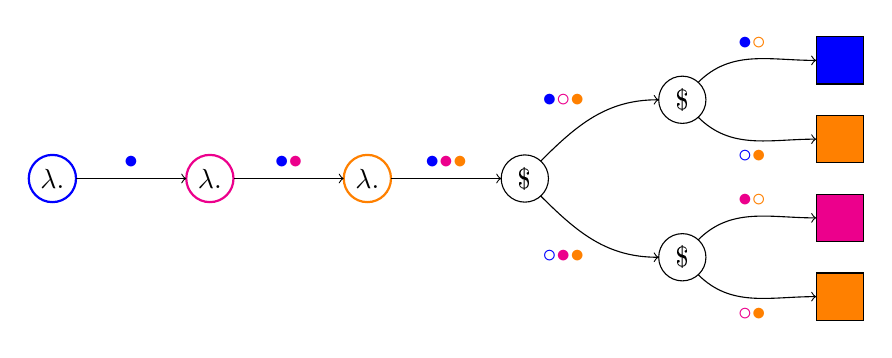
\begin{tikzpicture}
\draw[draw=blue   ,thick] (0,0) circle (.3cm) node[align=center] {$\lambda{}.$};
\draw[draw=magenta,thick] (2,0) circle (.3cm) node[align=center] {$\lambda{}.$};
\draw[draw=orange ,thick] (4,0) circle (.3cm) node[align=center] {$\lambda{}.$};

\draw (6,0) circle (.3cm) node[align=center] {\$};

\draw (8,1)    circle (.3cm) node[align=center] {\$};
\draw[fill=blue]   (10,1.5) +(-.3cm,-.3cm) rectangle +(.3cm,.3cm);
\draw[fill=orange] (10,.5)  +(-.3cm,-.3cm) rectangle +(.3cm,.3cm);

\draw (8,-1)    circle (.3cm) node[align=center] {\$};
\draw[fill=magenta] (10,-.5)  +(-.3cm,-.3cm) rectangle +(.3cm,.3cm);
\draw[fill=orange]  (10,-1.5) +(-.3cm,-.3cm) rectangle +(.3cm,.3cm);


\draw [->] (0.3,0)   to [out=0,in=180] node[above]{$\color{blue}{\bullet}$} (1.7,0);
\draw [->] (2.3,0)   to [out=0,in=180] node[above]{$\color{blue}{\bullet}\color{magenta}{\bullet}$} (3.7,0);
\draw [->] (4.3,0)   to [out=0,in=180] node[above]{$\color{blue}{\bullet}\color{magenta}{\bullet}\color{orange}{\bullet}$} (5.7,0);

\draw [->] (6.2,-.22)  to [out=-45,in=180] node[below left]{$\color{blue}{\circ}\color{magenta}{\bullet}\color{orange}{\bullet}$} (7.7,-1);
\draw [->] (6.2,.22)   to [out=45,in=180] node[above left]{$\color{blue}{\bullet}\color{magenta}{\circ}\color{orange}{\bullet}$} (7.7,1);
\draw [->] (8.2,1.22)  to [out=45,in=180] node[above]{$\color{blue}{\bullet}\color{orange}{\circ}$} (9.7,1.5);
\draw [->] (8.2,.78)   to [out=-45,in=180] node[below]{$\color{blue}{\circ}\color{orange}{\bullet}$} (9.7,.5);
\draw [->] (8.2,-.78)  to [out=45,in=180] node[above]{$\color{magenta}{\bullet}\color{orange}{\circ}$} (9.7,-.5);
\draw [->] (8.2,-1.22) to [out=-45,in=180] node[below]{$\color{magenta}{\circ}\color{orange}{\bullet}$} (9.7,-1.5);
\end{tikzpicture}
%</codebruijn>

%<*opening>
\begin{tikzpicture}
\draw (0,0)     circle (.3cm) node[align=center] {\$};
\draw (2.5,.75)   node[draw,dashed,regular polygon, regular polygon sides=3, shape border rotate=90]{$t_1$};
\draw (2.5,-.75)  node[draw,dashed,regular polygon, regular polygon sides=3, shape border rotate=90]{$t_2$};

\draw (-1,0)
  node[align=center]{$\color{blue}{\bullet}\color{orange}{\circ}\color{magenta}{\bullet}\color{teal}{\bullet}\color{lightgray}{\bullet}$} (1.7,1.5);
\draw [->] (.2,.22)  to [out=45,in=180]
  node[above]{$\color{blue}{\circ}\color{magenta}{\bullet}\color{teal}{\bullet}\color{lightgray}{\circ}$}
  (1.77,.75);
\draw [->] (.2,-.22) to [out=-45,in=180]
  node[below]{$\color{blue}{\bullet}\color{magenta}{\circ}\color{teal}{\bullet}\color{lightgray}{\bullet}$}
  (1.77,-.75);
\end{tikzpicture}
%</opening>

%<*opened>
\begin{tikzpicture}
\draw (0,0)       node[draw,diamond,align=center] {\$};
\draw (2.5,.75)   node[draw,dashed,regular polygon, regular polygon sides=3, shape border rotate=90]{$t_1$};
\draw (2.5,-.75)  node[draw,dashed,regular polygon, regular polygon sides=3, shape border rotate=90]{$t_2$};

\draw [->] (.23,.23)  to [out=45,in=180]
  node[above]{$\color{blue}{\circ}\color{orange}{\circ}\color{magenta}{\bullet}\color{teal}{\bullet}\color{lightgray}{\circ}$}
  (1.77,.75);
\draw [->] (.23,-.23) to [out=-45,in=180]
  node[below]{$\color{blue}{\bullet}\color{orange}{\circ}\color{magenta}{\circ}\color{teal}{\bullet}\color{lightgray}{\bullet}$}
  (1.77,-.75);
\end{tikzpicture}
%</opened>


Using a de Bruijn representation~\cite{MANUAL:journals/math/debruijn72} each
variable points to the binder that introduced it. Variables are finite numbers
(in the sense of \IdrisType{Fin}) counting the numbers of binders that separate
the variable from its binding site.

\ExecuteMetaData[Example.idr.tex]{scomb}
\ExecuteMetaData[UTLC.idr.tex]{scomb}


In a co-de Bruijn
representation~\cite{DBLP:journals/corr/abs-1807-04085} each subterm
selects exactly the variables that stay in scope for that term,
and so a variable constructor ultimately refers to the only variable still
in scope by the time it is reached.
%
This representation ensures that we know precisely what the scope of a given term
currently is.

We can recover terms living in arbitrary scopes by pairing a co-de Bruijn term
with a thinning~\cite{MANUAL:phd/nott/Chapman09}
embedding its tight support into the given englobing scope.
\todo{defined CdB}

\todo{application e.g. shrinking}

In order to efficiently represent and traverse terms in co-de Bruijn representation,
we need a compact encoding of thinnings and a cheap composition operator.
\todo{example: opening an application node}

The implementation of \typos~\cite{MANUAL:talk/types/Allais22} uses a co-de Bruijn
representation internally. \todo{explain why}
%
The developpement of the \typos{} language highlights a glaring gap between on the
one hand the experiments done in Agda and on the other the actual implementation
in Haskell.
%
The Agda-based experiments use inductive families that make the key invariants explicit
which helps tracking complex constraints and catches design flaws. The indices guarantee
that we always transform the thinnings appropriately when we add or remove bound variables.
%
The Haskell implementation represents a thinning as a pair of integers and resorts to
explicitly manipulating individual bits. It is not indexed and thus all the invariant
tracking has to be done by hand. This has led to numerous and hard to diagnose bugs.

\idris{} is a bootstrapped language. If we were to use such a co-deBruijn representation
of terms as a replacement for \idris{}'s current core language we would want, and should
be able, to have the best of both worlds: a safe and efficient representation!
